\chapter{Introduction}
\label{ch:intro}

Social insect societies are formed by thousands of individuals, which continuously move and interact with each other inside a dark nest. Honey bee colonies are thus organized complex and dynamical systems, which form a collective intelligence. Observing individual honey bees is, therefore, vital for understanding collective behavior, decision making, and organization of tasks within the colony.

Within the BeesBook project of the Biorobotics Lab of Freie Universität Berlin~\textcite{wario2015automatic} developed technologies to automatically track all individuals of a honey bee (Apis mellifera) colony. Shortly after birth, each bee has been marked on their thorax using circular 12-bit tags (figure~\ref{fig:markers}) and then added to the colony. The comb is observed by four cameras over a period of nine weeks and each picture is evaluated automatically. The resulting data set contains the position of each bee and its decoded id.

In this thesis, temporal interaction networks, based on spatial proximity, are derived from the described data set. Each node in the network is a bee and a link between two individuals is created if they share a position close to each other. Social network analysis methods are applied to determine the usefulness and the characteristics of the resulting networks and its communities.

Until now, social network analysis has been applied to only a subset of a honey bee colonies live, simply because the data were not available to this extent and quality so far.

\begin{figure}[htb]
	\centering
	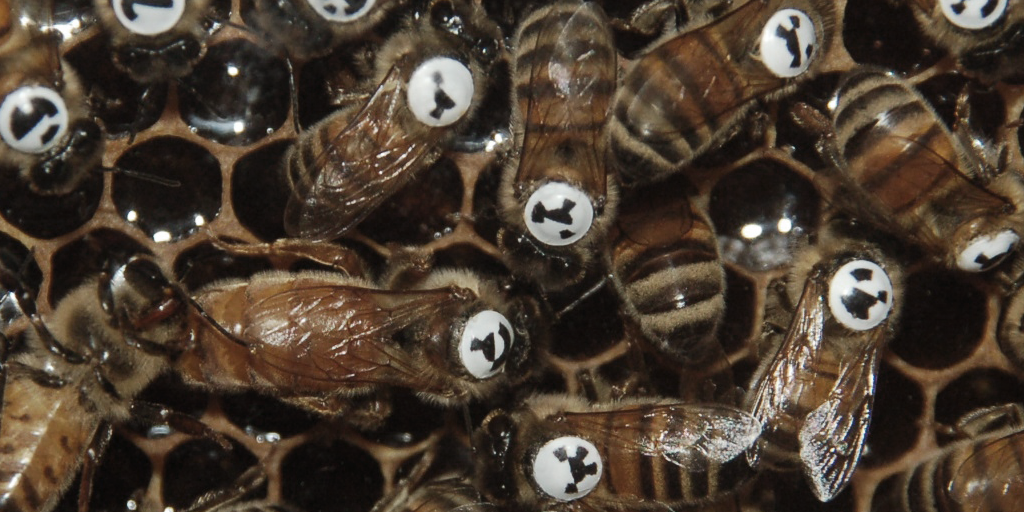
\includegraphics[width=1.0\textwidth]{Figures/markers}
	\caption{Tagged bees inside the hive.}
	\label{fig:markers}
\end{figure}

\section{Motivation}
[TODO weitermachen]
Most of the studies analysing behaviour of insects colonies only use a small amount of individually labeled animals, a short observation period, and usually manually detect interaction between animals looking at the videos. data~\cite{quevillon2015social}[TODO: more references]. Here it is done in a more inclusive way, all animals, long term observation, automatic detection of individuals.

Conventional approaches usually focus on a small subset of the hive life, whether this regards time, space, or animal identity[TODO: change sentence]. A subset in terms of recording time (short observation period), space (only parts of the hive are observed), number of individuals (only some individuals are observed). 


\section{Research Goal}

The aim of this thesis is to investigate whether the provided data set of tracked honey bees is useful for creating worker-worker interaction networks using spatial proximity as a proxy for interactions between bees. Thus, I need to implement a pipeline to infer networks out of the data set. Furthermore I want to find out if the resulting networks are suitable for social network analysis.

I want to achive my research goal by answering the following questions:

\begin{enumerate}
\item \emph{Is it possible to infer networks with the provided data set?}\\
What challenges and limitations does the data set imply?
\item \emph{What kind of networks emerge and what are their properties?}\\
How are those networks characterized in and are they different from a random network?
\item \emph{Do community structures exists?}\\
Are those communities robust?
\item \emph{How are those communities characterized?}\\
Do they reflect known colony behaviour in terms of age and spatial distribution?
\item \emph{How do the communities evolve over time?}\\
Are they stabel over time and how do members change communities over time?

\end{enumerate}


\section{Methodology}

Network Science Approach.

\section{Outline}
[TODO]